\chapter{Grundlagen}
\label{ch:Grundlagen}

\todo[inline]{Schreiben der Einführung des Kapitels \ref{cha:grundlagen} Grundlagen}

\section{Verstärkendes Lernen(Reinforcement Learing)}
Verstärkendes oder auch Bestärkendes lernen beschäftigt sich mit dem Problem, dass ein eigenständiger Agent innerhalb einer unbekannten Umgebung lernen soll, welche Folgen seine Aktionen hinsichtlich der Zustände der Umgebung haben werden. Dem Agenten steht eine begrenzte Anzahl von Aktionen zur Verfügung. Zum Beispiel bewege dich nach oben, unten, rechts oder links. Der Agent lernt also, dass die Aktion 'bewege dich nach oben' einen Ausgangszustand in einen neuen Zustand transformiert. Führt der Agent die Aktion 'bewege dich nach oben' aus, dann ist jedoch die Zustandsveränderung abhängig von der individuellen Umgebung in der sich der Agent befindet. Unter Umständen ist es in dieser speziellen Umgebung nicht möglich sich von dem aktuellen Zustand, in der sich der Agent aktuell befindet, in einen Zustand zu bewegen der 'oberhalb' des Agenten liegt, denn es könnte eine Mauer direkt oberhalb des Agenten sein. Der neue Zustand wäre also der alte Ausgangszustand. Das bedeutet für den Agenten, dass er genau differenzieren muss in welchem Zustand er welche Aktion durchführt. Warum sollte ein Agent jedoch eine Aktion in einem bestimmten Zustand nicht durchführen und wann sollte er eine Aktion durchführen? \\

\begin{figure}[!htbp]
  \centering
  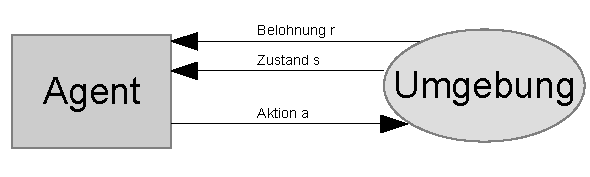
\includegraphics[scale = 1]{inhalt/abbildungen/agent_umgebung.pdf}
  \caption{Der Agent und seine Wechselwirkung mit der Umgebung}
  \label{fig:agent_umgebung}
\end{figure} 

Die Antwort liegt in dem durch Belohnung und Bestrafung antrainierten Verhalten des Agenten.

Die Abbildungen dieses Hauptproblems ähneln sich in der Literatur sehr stark, die Abb. 16.1 \cite[398]{Alpaydim} und die Abb. 10.4 \cite[290]{Ertel} sind nahezu identisch.

Im Gegensatz zu den Lernverfahren beim überwachten Lernen fehlt dem Agenten beim verstärkenden Lernen ein 'Lehrer' der dem Agenten genau sagt ob seine Aktion richtig oder falsch ist. Ein überwachtes Lernverfahren wird zuerst mittels eines Trainingssets kontrolliert belehrt. Das Trainingsset für ein überwachtes Lernverfahren besteht aus verschiedenen Eigenschaften(Features) und einer den Eigenschaften zugeordneten Klasse beziehungsweise Zielvariable(Target Variable). Abbildung \ref{fig:vogel_spezies} zeigt, wie so ein Trainingsset aussehen könnte\cite[8]{Harrington}. Die Spalten Gewicht, Flügelspanne, Schwimmhäute und Rückenfarbe sind die Eigenschaften und die Spalte Spezies beinhaltet die Zielvariablen. Das überwachte Lernverfahren lernt mittels des Trainingsdatensets die Beziehungen zwischen den Eigenschaften und der Klassen.   \\

\begin{figure}[!htbp]
  \centering
  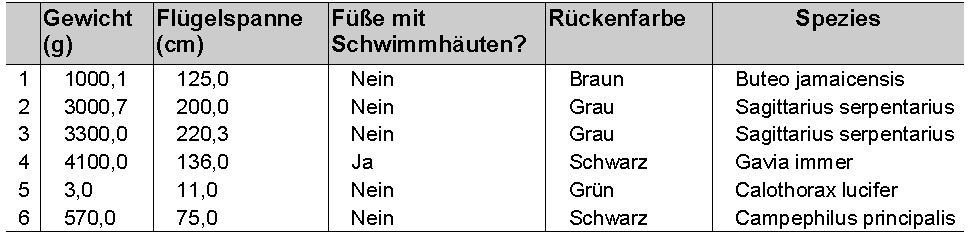
\includegraphics[scale = 0.89]{inhalt/abbildungen/vogel_spezies.pdf}
  \caption{Vogelspezies Klassifikation basierend auf vier Eigenschaften}
  \label{fig:vogel_spezies}
\end{figure} 

Verstärktes Lernen umfasst die Probleme, bei denen in der Regel kein solches Trainingsdatenset vorliegt, welches genau festlegt ob eine Aktion in einem Zustand korrekt oder falsch ist. Meistens ist dem Agenten vorher nicht bekannt welche Auswirkungen seine Aktionen auf die Umwelt haben werden. Verstärkendes Lernen kann trotzdem vom überwachten Lernen profitieren, denn es ist möglich den Agenten in der Anfangsphase des verstärkten Lernens explizit zu programmieren und ihn dadurch auf bestimmte Auffälligkeiten oder Muster aufmerksam zu machen. Ist es zu schwierig dies explizit zu programmieren, dann kann auch ein Mensch dem Agenten die richtigen Aktionen vorgeben. Sehr nützlich werden diese beiden Unterstützungen der Anfangsphase des verstärkenden Lernens, sobald die Dimensionen der Umwelt oder des Agenten eine bestimmte Größe überschreiten. Eine Aktionsdimension kann sehr wenige Aktionen beinhalten zum Beispiel die vier Aktionen bewege dich nach oben, unten, rechts oder links. Roboter die dem Menschen nachempfunden sind verfügen über bis zu 50 verschiedene Motoren für die einzelnen Gelenke. Diese müssen gleichzeitig angesteuert werden, was zu einem 50-dimensionalen Zustandsraum und einem 50-dimensionalen Aktionenraum führt\cite[305\psq]{Ertel}.

\subsection{Die drei Arten des maschinellen Lernens}
\label{subsec:Die drei Arten des maschinellen Lernens}

\myparagraph{Überwachtes Lernen}

Verfahren aus der Gattung des überwachten Lernens,  benötigt Datensets mit bestimmten Eigenschaften. Ein überwachter lernfähiger Algorithmus zur Klassifizierung von Daten, benötigt ein Trainingsset bestehend aus Eigenschaften(Features) und den dazugehörigen Klassen bzw. Zielwerten(Target Values). Abbildung \missingfigure{Erstellen eines Trainingssets für überwachte Klassifizierung} stellt ein Beispiel für ein mögliches Trainingsset dar. Ziel der Klassifizierung ist das vorhersagen von Zielwerten. Die Qualität der Zielwerte kann mittels Testsets ermittelt werden. Ein Testset ist ein Datenset bestehend aus Eigenschaften ohne die dazugehörigen Klassen.

\myparagraph{Unüberwachtes Lernen}

\myparagraph{Bestärkendes Lernen}
Bestärkendes Lernen oder verstärkendes Lernen(engl. Reinforcement Learing) ist 

\section{Spielentwicklung}

\section{Lineare Algebra}

\section{Heuristik}